\documentclass[%
 aip,
% jmp,
% bmf,
% sd,
% rsi,
 amsmath,amssymb,
%preprint,%
 reprint,%
%author-year,%
%author-numerical,%
% Conference Proceedings
]{revtex4-1}

\usepackage{graphicx}% Include figure files
\usepackage{dcolumn}% Align table columns on decimal point
\usepackage{bm}% bold math
%\usepackage[mathlines]{lineno}% Enable numbering of text and display math
%\linenumbers\relax % Commence numbering lines

\usepackage[utf8]{inputenc}
\usepackage[T1]{fontenc}
\usepackage{mathptmx}
\usepackage{etoolbox}

%PW additional packages
\usepackage{braket}
\usepackage{todonotes}

%% Apr 2021: AIP requests that the corresponding 
%% email to be moved after the affiliations
\makeatletter
\def\@email#1#2{%
 \endgroup
 \patchcmd{\titleblock@produce}
  {\frontmatter@RRAPformat}
  {\frontmatter@RRAPformat{\produce@RRAP{*#1\href{mailto:#2}{#2}}}\frontmatter@RRAPformat}
  {}{}
}%
\makeatother
\begin{document}

\preprint{AIP/123-QED}

\title[MRChem]{The MRChem MRA code for molecular electronic calculations. Performance and scaling properties}
\author{Peter Wind}
\affiliation{Department of Chemistry, UiT - The Arctic University of Norway, N-9037 Tromsø, Norway}
\author{Magnar Bjørve}
\affiliation{Department of Chemistry, UiT - The Arctic University of Norway, N-9037 Tromsø, Norway}
\author{Anders Brakestad}
\affiliation{Department of Chemistry, UiT - The Arctic University of Norway, N-9037 Tromsø, Norway}
\author{Gabriel Gerez}
\affiliation{Department of Chemistry, UiT - The Arctic University of Norway, N-9037 Tromsø, Norway}
\author{Stig Rune Jensen}
\affiliation{Department of Chemistry, UiT - The Arctic University of Norway, N-9037 Tromsø, Norway}
\author{Roberto Di Remigio Eikås}
\affiliation{ENCCS Department of Information Technology, Uppsala University, Uppsala, Sweden}
%To check Roberto affiliation
\author{Luca Frediani}
\affiliation{Department of Chemistry, UiT - The Arctic University of Norway, N-9037 Tromsø, Norway}




\date{\today}

\begin{abstract}
MRChem is a MRA code for molecular electronic structure calculations, based on a multiwavelets adaptive basis representation. A description of the implementation strategy is provided. Benchmark calculations on systems comprising more than thousand orbitals at the HF level are analyzed, with an emphasis on scaling properties. 
We show that some terms which formally scale as $~0(N^2)$, in effect have a better scaling because of the implicit screening introduced by the inherent adaptivity of the method. Comparison with traditional GTO based software, show that MRChem can be competitive with respect to computation time.

\end{abstract}

\maketitle

\section{Introduction}


GTO and more generally MRA are well established as a standard for \emph{ab-initio} molecular electronic structure calculations. As their shape is closely related to the electronic structure of atoms, even very small basis sets (a few functions per orbital) can give reasonable results for describing molecular properties. However for extended systems the description of each orbital still requires the contributions from the entire basis in order to ensure orthogonality. Even when using localized orbitals, a large proportion of the coefficients will be very small for those systems.

In a MRA framework, the basis can adapt according to the function described (for an in-depth review of the MRA method in the field of Quantum Chemistry, see \citep[]{bischoff2019}). The available basis is in principle infinite and complete, and the basis actually used is dynamically adapted to the local shape of the function and the required precision. However reasonable results can require the real-space basis to comprise millions of elementary functions for each orbital. In this sense, the method starts with a big handicap, compared to Gaussian basis sets.

The challenge is not only the large amount of operations needed to perform any mathematical transformation in this approach, but also the large memory footprint: beyond a certain system size, not all data can be stored in local (i.e. fast access) memory. On modern computers, data access is generally more time consuming than the mathematical operations itself, especially if the data is not available locally. The implementation must be able to efficiently copy large amounts of data between compute nodes and the algorithm must be devised so as to use or reuse the data already locally available when possible.

With the exponential development of available computational resources, it has now become possible to perform such MRA calculations on systems comprising 
thousands of atoms \cite{ratcliff2020}, \cite{madness2016}. 

In this article, we will present the main implementation features of a MRA code, MRChem, which is capable of describing such large systems at the Hartree Fock or Density Functional Theory (DFT) level.  

The large memory requirement is addressed by storing the data in a distributed "memory bank", where orbitals can be sent and retrieved independently by any CPU. The total size of the memory bank is then only limited by overall memory available on the entire computer cluster.

The large computational cost is addressed by parallelization either at the orbital level or through real space partitioning. This dual strategy allows to minimize the relative cost of communication and the overall computational costs. Further the most computational intensive parts are expressed as matrix multiplications, which allows for optimal efficiency.  

The multiwavelet approach adapts the precision to the "smoothness" of the potential in a continuous way. The potential resulting from remote subsystems will locally be "smooth" and thereby only require a simplified (coarse grid) description. 

Using localized orbitals the adaptivity of the multiwavelets description will significantly reduce the computational effort required to compute the terms involving remote orbitals. This opens the way for a linearly scaling method where the linearity arises naturally from the methodology, rather than being obtained by specific additional methods such as multipole interactions or purification of the density matrix \cite{trygve}.

Benchmark calculations at the Hartree Fock level show that MRChem is able to describe systems with thousands of electrons, exhibits near-linear scaling properties and can also be competitive with state-of-the-art electronic structure software based on LCAO methods.


\section{Solving the Hartree-Fock and Kohn-Sham equations with Multiwavelets}

We consider the SCF equations common to the HF method and the KS equations of DFT:

\begin{equation}\label{eq:differential-scf}
  \left( -\frac{1}{2}\nabla^2 + V \right) \psi_i = \sum_{j_{occ}} F_{ij} \psi_j
\end{equation}

where the Fock matrix elements $F_{ij}$ are obtained as
\begin{equation}\label{eq:fock-matrix-definition}
  F_{ij} = \braket{ {\psi_i}|{-\frac{1}{2}\nabla^2+V}|{\psi_j}}
\end{equation}

In the above equations, $T = -\frac{1}{2}\nabla^2$ is the kinetic energy operator, and the potential $V$ contains the nuclear-electron attraction $V_{nuc}$, the Coulomb repulsion $J$, the exact exchange $K$ and, in case of DFT, the exchange and correlation potential $V_{XC}$. 

To solve the SCF equations within a MW framework, it is necessary to rewrite the differential equation \ref{eq:differential-scf} as an integral equation:
\begin{equation}\label{eq:integral-scf}
\psi_i = -2 H^{\mu_i}\left[V\psi_i - \sum_{j_{occ} \ne i} F_{ij} \psi_j\right]
\end{equation}
This is obtained by recalling that the shifted kinetic energy operator $T-\epsilon$ has a closed-form Green's function:
\begin{equation}\label{eq:helmholtz-green}
    (T-\epsilon)^{-1} = 2 H^{\mu}(r) \quad H^{\mu}(r) = \frac{e^{-\mu r}}{r} \quad \mu = \sqrt{-2\epsilon} 
\end{equation}
%Working in the integral form is both a necessity and an advantage. %\todo[inline]{PW: I do not see why it is an advantage; it would be much easier if we could use a basis with an exact second order derivative}

A multiwavelet representation does not have a predefined basis, and as such it is not possible to express functions and operators as vectors and matrices of a predefined size and the virtual space is to be regarded as infinite, although each function has a finite, truncated representation defined by the chosen precision threshold. It is therefore necessary to have working equations which allow the direct optimization of orbitals.
At the same time one deals only with occupied orbitals and the Fock matrix in Equations \ref{eq:differential-scf} and \ref{eq:integral-scf} is therefore limited in size. 

Differential operators such as the Laplacian, also pose a fundamental problem for function representations which are not continuous, and a naive implementation leads to numerical instabilities. Robust approximation are nowadays available\cite{der-paper}, but for repeated iterations avoiding the use of the Laplacian operator is still an advantage. 

%\todo[inline]{PW: The "preconditioner" is only useful if it accelerate the convergence. The ideal (or at least exact to second order) preconditioner is the inverse of the Hessian. In traditional methods one use good approximations for the inverse Hessian (diagonal or so), while the "preconditioner" we use is only a matrix that we put in front because it is the only way we can practically solve the equation, but is not optimized for being a good approximation of the inverse Hessian. I have therefore rewritten the text below}

Additionally, it can be shown that iterating on the integral equation corresponds to a preconditioned steepest descent. Practical applications show that this approach is comparable in efficiency (as measured in the rate of convergence of the SCF iterations) to more traditional methods [REF?]. 

\subsection{The basic operations in the SCF iterations} %put complex conjugates!

For a detailed description of the SCF optimization using Multiwavelets, the reader is referred to a recently published article which describes the algorithm in detail [REF].

We will here list the main operations, with emphasis on those aspects which are relevant for an efficient parallelization.

The starting point is an initial set of orthonormal orbitals which define a Slater determinant for the given problem. A density is computed and the corresponding operators ($J$, $K$ and $V_{XC}$) are built. The Fock matrix (Eq.~\ref{eq:fock-matrix-definition} is computed. This requires the application of the kinetic operator ($T$), nuclear  potential ($V_{nuc}$), Coulomb operator ($J$), and  the exchange potential ($K$) and/or the "exchange-correlation" potential from the density functional ($V_{xc}$) on each occupied orbital. The argument for the application of the integral operator is assembled (the square bracket in Eq.~\ref{eq:integral-scf}). Then the integral operator is applied and the cycle is iterated after a normalization step. 

The elementary operations required for all those operations are
\begin{itemize}
\item Construction of a MW function given an analytic or sampled function.
\item Evaluation of the value of MW functions at a given point in space.
\item Multiplication of a function by a number.
\item Sum of two MW functions.
\item Product of two MW functions.
\item Computation of the overlap integral between two MW functions.
\item Application of a potential on a MW function (multiplication).
\item Evaluation of the first order derivative of a MW function.
\item Application of Coulomb operator on a MW function to obtain an electrostatic potential.
\item Construction and application of the Helmholtz operator.
\end{itemize}


All these operations are provided by the MRCPP library\cite{mrcpp} and must be composed to achieve a SCF implementation, and they must be integrated in a parallel framework to achieve good scaling and performance.

In addition, the SCF cycle requires schemes for orbital orthonormalization, rotation, and localization, Fock matrix diagonalization, history storage and utilization to enable KAIN acceleration.~\cite{kain}

\subsubsection{$T$}
The application of the kinetic operator on a MW function is formally not well defined. However, it is possible to compute first derivatives provided repeated applications are avoided. The matrix elements of the kinetic energy operator can therefore be computed as:
\begin{equation}
  T_{ij} = -\frac{1}{2} \braket{\nabla \psi_i | \nabla \psi_j}
\end{equation}
Computing the matrix elements require therefore only the gradient followed by the inner product. This last step ensures that the resulting number is in practice accurate enough.\cite{derivative-paper}

\subsubsection{$V_{nuc}$}

\todo[inline]{I'm not quite sure I have understood this explanation...}
\todo[inline]{PW: it is more explicit now, better?}

The application of the nuclear potential (and possibly any additional external field) can be performed in two ways. Either the sum over nuclei is performed as a sum of matrix elements for the individual nuclei:
\begin{equation}
  V_{nuc} \phi_j = \sum_{k = nuclei} (V_k \phi_j)
\end{equation}

or the sum over the potentials is performed first, and the matrix elements evaluated at the end:
\begin{equation}
  V_{nuc} \phi_j = (\sum_{k = nuclei} V_k) \phi_j
\end{equation}
In our present implementation, the second form is used.

The total potential for all nuclei ($\sum_{k} V_k$) can be very large in terms of memory. It describes the potential over the entire space, whereas only the parts that overlap with the occupied orbitals are actually used. In the future we plan to adapt the accuracy according to the electronic density.

%The first expression is requires less operations, since only one operator application needs to be evaluated. The second form requires to apply an operator for each nucleus.

%However the second form may still have computational advantages:  The second form is also simpler to set into a parallel framework, since the contribution from each nucleus can be evaluated completely independently. The potential for a single nuclei is memorywise smaller than the total potential.

%I %but we should do something about it to reduce or delocalize the memory footprint

\subsubsection{The Coulomb potential $J$}

The coulomb interaction is computed in two steps. First the total density is obtained as a sum of orbital contributions. Thereafter the Coulomb potential is computed by applying the Poisson kernel.
\begin{eqnarray}
  \rho(r) &= \sum_k \phi^*_k(r)\phi_k(r)\\
  J(r) &= \int \frac{\rho(r')}{|r-r'|} \, dr'
\end{eqnarray}

\subsubsection{The exchange potential $K$}

The exchange potential is the most computationally demanding part, because it cannot be written in closed form. A Coulomb potential must be constructed and applied for each orbital pair:

\begin{equation}
  K \phi_j = \sum_k  K_k \phi_j 
\end{equation}
with 
\begin{equation}
  K_k \phi_j = \phi_k(r) \int \frac{\phi^*_k(r')\phi_j(r')}{|r-r'|} \, dr'
\end{equation}

Section \ref{Xscreen} provides a more detailed description of how these terms can be evaluated efficiently in a MRA framework. 

\subsubsection{$V_{xc}$}
\todo[inline]{PW: "each point in space" is not very correct. Should be "at the same resolution as the used basis". Reformulate? }
The density is evaluated at each point in space, and the exchange and correlation potential $V_{XC}$ is then evaluated using the external library XCfun[REF], and transformed back into a MW potential.

\subsubsection{Helmholtz operator}

The Helmholtz operator defined in Eq.~\ref{eq:helmholtz-green} and employed in Eq.~\ref{eq:integral-scf}, depends on the orbital energy. As such one needs to construct as many operators as there are orbitals.

%\subsection{MRChem software, MRCPP and Vampyr}
%section about availability and things the code can do for the user
%\todo[inline]{Do we nee this at all?}
%\todo[inline]{PW: probably not if there is a reference to another paper where this is shown}

\section{Implementation details and parallelization strategy}

MW calculations can be computationally demanding. Both the total amount of elementary operations, the large amount of memory required and the capacity of the network are important bottlenecks. 

In practice a supercomputer is required for calculations on large systems.
For example the representation of one orbital is described typically by of the order of 10-500MB of data (see section \ref{sizes}). Usually several sets of orbitals are required in the scf process (previous iterations, right hand size of equations etc.). If 1000 orbitals are described, this will often require more memory than is locally available on a single compute node in a cluster. Therefore it is required to store the data in a distributed way. At the same time, the equations require to access all pairs of orbitals, i.e. all the data must at some point be accessible locally.

In order to solve the equation in parallel, the problem needs to be partitioned into smaller parts that can be computed with as little transfer of data as possible between the different parts.



\subsection{Localized versus canonical orbitals}

Although localized and canonical orbitals represent the same N-electrons wave function, the numerical operations required to solve the equations will have different scaling properties in a canonical or localized representation.
Because of the inherent adaptiveness of the MW approach, multiplying two orbitals, or applying an operator onto an orbital can be done more efficiently if the orbitals are localized in space. Even if the orbitals have non-negligible values in a large portion of space, the adaptiveness properties will make sure that the calculations in the parts where the orbitals are small are done at a coarser level of accuracy, and therefore faster than in the regions with larger values.

\subsection{Local (real space) versus orbital representation}
%NB: easy to confuse real space local and localized orbitals!

The orbitals need to be stored on the computer. This can be done in several ways. The KS or HF equations are written in terms of orbitals, and therefore it is natural to implement the code in a way that follows the mathematical expressions, i.e. each orbital is stored individually. Another way of partitioning the problem, is to consider one part of real space at a time, and store together the contributions from all the orbitals at that position. Both approaches have advantages and disadvantages.

We will show here why it is advantageous, for some terms at least, to shift to a real-space partitioning approach.

(This is similar to the history for gaussian basis set methods, which started using Molecular Orbitals, but for large systems could get more efficient implementations by expressing the core terms using an "Atomic Orbitals" representation \cite{trygve})

In the computation of the Fock matrix elements, one has to evaluate terms of the form 
%note: the equation is not interpreted right by overleaf if physics package is used
\begin{equation}
  {\hat O}_{ij} = \braket{\phi_{i} | {\hat O} |\phi_j}  = \braket{\phi_i | {\hat O} \phi_j} 
\end{equation}

where $\phi_i$ and $\phi_j$ are occupied orbital, and ${\hat O}$ is an operator, for example the nuclear potential operator. If the application of the operator is considered as a $~0(N)$
%not if the operator grows with N. Not that simple!
operation, the calculations of the entire matrix runs over all the orbital pairs and therefore scales formally as $~0(N^2)$. We can express explicitly the orbitals in the multiwavelet basis:

\begin{equation}
  \phi_i = \sum_{k,n} c_{ikn} p_{kn} 
\end{equation}
\begin{equation}
  {\hat O} \phi_j = \sum_{k,n} d_{jkn} p_{kn} 
\end{equation}

where $p_{kn}$ is a member of the used MW basis, i.e. a three-dimensional polynomial (index $k$) for a multiwavelet node (index $n$) at specific position in space, and $c_{ikn}$ are the coefficients that define the function $\phi_i$ in that basis. 

Since the basis is adaptive, different functions will use different sets of nodes. 
In order to compute the overlap of two functions $\phi_i$ and ${\hat O} \phi_j$, they are first adaptively projected onto a common basis and multiplied:

\begin{equation}
  \braket{\phi_i|{\hat O} \phi_j} = \sum_{k,n} c_{ikn}d_{jkn}
\end{equation}

since $\braket{p_{kn}|p_{lm}} = \delta_{kl}\delta_{nm}$

This operation is equivalent to the multiplication of the $c$ and $d$ matrices. However for large systems, it is not possible to hold the coefficients for all the indices i,j,k,n in local memory.
The "MO" approach is then to sum over all $k,n$ for each pair ij independently. The problem is that each coefficient $c_{ikn}$ is used only once at a time. On modern based computers memory access are much more time demanding (factor of the order of 100 for most CPU based systems) than the mathematical operations itself.  A much faster implementation is to consider a specific node n and perform the product for all i, j and k values within this node. 

\begin{equation}
\label{equ:sum}
  \braket{\phi_i | {\hat O} |\phi_j}_n = \sum_{k} c_{ikn} d_{jkn} \forall i,j
\end{equation}

This results in a series of independent matrix multiplication operations that can fully utilize the capabilities of the computer. 

This means however that the storage of the orbitals in memory must be adapted. Instead of storing each orbital separately (orbital or MO representation), the values of all the orbitals at specific positions in space (node) must be easily accessible (local representation). To change from an orbital to a local representation is a $~0(N)$ operation,

It is still possible, to take advantage of the screening in the local approach: for each function, the norm values within each node is stored, so that when the product of the norms is below a threshold, the corresponding matrix multiplication does not need to be performed.

Also orbital rotations can be addressed in a similar way.

%which terms are using local storage



\subsection{Adaptivity}

In the MRA framework, the required precision can limit the number of elementary operations at several levels.

At the lowest level, most operations on a function in a multiwavelet representation will successively refine the local basis (i.e. grid) of the resulting function, until the required precision is reached. That means that the computational effort required will vary according to the position and shape of the functions or operators. For example the product of two functions which are localized in different part of space, will normally be done faster than the square of one of them. [REF?]

At a higher level, only the parts of functions with absolute value (norm of the node) above a defined threshold can be retrieved before even processing them; this is used in the scheme presented in the previous section.

Finally at the coarsest level, one can start to perform a SCF calculation with low precision, and use the final result as starting guess for a calculation with higher precision. In contrast to finite basis sets (which usually are not subsets of each others), a multiwavelet function represented with a given precision, can directly be used as a valid representation at a different precision.


\subsection{MPI parallelization}

MRChem is parallelized using Message Passing Interface (MPI \cite{mpi}) and OpenMP \cite{omp}.  

The MPI processes are partitioned into three groups:

\subsubsection{MPI "workers"} 
They perform the mathematical operations. These processes have also access to multiple threads for OpenMP parallelization. The large majority of the cores are assigned to worker processes.

The low level operations (on one or two orbitals or MW trees, and on nodes) are included  in the MRCPP library. The MRCPP will perform tree operations as a set of operations on nodes. Those operations will then be performed in parallel by OpenMP threads. The thread parallelity is transparent for the library user; only the number of threads needs to be set.


\subsubsection{Memory bank processes} 
These processes are only receiving and distributing data to the workers, they do not perform major mathematical operations and are not threaded. Those processes will impose a high load on the network; it is therefore important to distribute those process on all compute nodes in order to avoid saturation of the local network. Since the memory bank processes are different from the worker processes, the worker processes can access all the data without direct communication with other workers (in effect, one sided memory access). Efficient transfer of data is the key to a successful parallelization scheme.

In the multiwavelet approach, orbitals are functions represented in a tree structure. The root nodes cover the entire space of the system, and each subdivision defines branches. In order to facilitate the transfer of those functions, the tree structure and the node data are stored in piecewise contiguous memory. This allows the data to be sent efficiently among MPI processes: only the position in memory of the start and end of the pieces are required, and some metadata information. A tree can then be transfered without intermediate buffering and with little overhead. 
The MRCPP library contains functionalities to easily and efficiently transfer MW trees (or orbitals) between MPI processes. 

The interface is simple and intuitive, and the basic commands in the C++ code are:
\begin{itemize}
    \item Save Orbital, give it an identification tag "id": 
    
put\_orb(id, Orbital)
\item Fetch Orbital with  identification tag "id": 

get\_orb(id, Orbital)

\end{itemize}


The underlying libraries will then find a suitable place in the "bank" to store the orbital.

%The MRCPP library allows to store a function as "shared memory" using MPI-3 functionalities. In such a format, all the MPI processes on a compute node can directly access a function using only one copy on the compute node. In our present implementation, the Nuclear and Coulomb potentials are stored in shared memory form.
%(We did not use the shared memory feature as much as intended, because we noticed that it sometimes causes a drop in performance, that was difficult to understand and control.)

\subsubsection{Task manager} 
In a localized orbital approach, many of the elements of the matrix $\braket{\phi_i|{\hat O} \phi_j}$ will be small. Since the method is inherently adaptive using the MRCPP library, the small elements will be faster to compute. In order to fully exploit this feature, a dynamical distribution of tasks is required.  
In practice the matrix $\braket{\phi_i|{\hat O} \phi_j}$ is partitioned into blocks. Each block represent one task to be performed by a "worker". In a local representation, each node is simply assigned to a separate task. When a "worker" is done with one task it can ask for a new task from the "task manager" until all the tasks are completed.

One single MPI process is reserved for managing the task queue. The only purpose of this process is to keep account of the tasks that have been assigned and the tasks left, and distribute unsolved tasks to the workers. It does only send and receive small amounts of data at a time (a few bytes) and will therefore in practice not be saturated with requests.



%In a fixed and limited basis set, the functions and operators can be represented as dense arrays, and the mathematical expressions become matrix multiplications. Matrix multiplication can be performed very efficiently on all types of supercomputers (both CPU and GPU based).
%In the multiwavelet representation, the representation of functions are given in a different basis, and there is no simple way to represent the equations as dense matrix multiplications. Only at the node level, the polynomial representation is in a predefined basis, and this is exploited, but there are still too few polynomials to fully take advantage of the hardware. 

%in appendix? example of C++ command to fetch and store orbitals?

\subsection{Exchange screening}
\label{Xscreen}

The exchange terms require the evaluation of

\begin{equation}
\label{equ:ex}
  K_{Ex}^k(r) \phi_j = \phi_k(r) \int \frac{\phi^*_k(r')\phi_j(r')}{|r-r'|} \, dr'
\end{equation}

 for all $k$ and $j$

The evaluation of equation (\ref{equ:ex}) can be divided into 3 operations:
\begin{itemize}
\item Product of $\phi^*_k(r')$ and $\phi_j(r')$
\item Application of Poisson operator, $\int \frac{(\phi^*_k(r')\phi_j(r'))}{|r-r'|} \, dr'$
\item Product with $\phi_k(r)$, $\phi_k(r) (\int \frac{\phi^*_k(r')\phi_j(r')}{|r-r'|} \, dr')$
\end{itemize}

The application of the Poisson operator gives a long range potential that decreases as 1/r. However if the function $\phi_k(r)$ is localized, only the the part of the potential where $\phi_k(r)$ is large enough needs to be computed. More precisely the accuracy of the potential needs only to be computed up to a precision which is inverse proportional to the value of $\phi_k(r)$ at that point. 

To handle this situation, the Poisson operator can use an adaptive precision, where the required precision of the operator application is determined locally by the value of a given function. In practice, a set of functions can be provided, and the precision at a given node is determined by the largest value of the norm of those functions at this node. This allows to treat the two terms $\phi_k(r) \int \frac{\phi^*_k(r')\phi_j(r')}{|r-r'|} \, dr'$ and  $\phi_j(r) (\int \frac{\phi^*_k(r')\phi_j(r')}{|r-r'|} \, dr')$ using the same $\int \frac{\phi^*_k(r')\phi_j(r')}{|r-r'|} \, dr'$.  Also complex functions can take advantage of this symmetry, since the complex and real part of $\phi_k(r)$ can then use the same $\int \frac{\phi^*_k(r')\phi_j(r')}{|r-r'|} \, dr'$.

Without screening, the number of exchange terms grows as $N^2$ and each term requires the application of Poisson operator. Distant orbitals that do not overlap, do not contribute, and therefore proper handling of the screening will be reflected in a cost of the exchange terms that grows linearly in size for large enough systems (if the required overall absolute precision is held constant). 

In practice if the product of $\phi^*_k(r')$ and $\phi_j(r')$ is small enough, the calculation of the corresponding term can be interrupted. As is shown in section \ref{sec:screen} this leads to an effective long range screening.


\subsection{$0(N_{occ}^3)$ terms}

In our implementation there are two steps which require a number of terms that scale with the third power of the number of (occupied) orbitals. 

The localization algorithm involves the product of dense matrices with sizes $N_{occ} \times N_{occ}$. 

The scheme for orthogonalization of orbitals uses the diagonalization of a hermitian matrix and subsequent matrix multiplications which both scale as $0(N_{occ}^3)$

Dense matrix operations can be performed extremely effectively on any computer, and those terms will not contribute significantly to the total computation time before considering sizes larger than roughly $N_{occ}=1000$ for serial matrix multiplications, or 10 to 100 thousand for parallel matrix multiplications (not yet implemented). 

Both steps are not specific to the multiwavelet approach, on the opposite, basis set approaches may require those steps to be performed on the virtual orbitals too. For large systems, it might also be possible to exploit the numerical sparsity of the matrices.

% In standard approaches the total number of basis functions has to be considered in the diagonalization steps ($0(N_{basis}^3)$). ?
% or ($0(N_{occ}^2 N_{basis})$ ? as claimed in
% The Journal of Chemical Physics 140, 204110 (2014); doi: 10.1063/1.4871876

\section{Benchmark results}
%\todo[inline]{PW: need to explain precision notation mw4, mw5...}
In this section we will show how MRChem performs for some simple systems of different size. MRChem is still under development and the results shown here are just a snapshot of the present situation. The goal is not to determine the limitations of the model, but rather to show that at least in some cases it behaves as intended and that the development is going the right way.

All the benchmark runs presented here were performed on "Betzy", a BullSequana XH2000 computer cluster, with 128 cores and 256 GiB memory per compute node, and infiniband HDR 100 interconnect REF?.

All times given in this section are subject to a significant imprecision. The reasons for this are multiple. The runs have been executed in a MPI parallel framework on a supercomputer shared with other users. Several algorithms are performed with dynamic allocation of tasks; as a consequence the same calculations can have a different workload distributions in two repeated identical runs. The network capacity may also be affected by other users. In addition the time spent in different parts of the code may not be well defined: in a parallel framework the same code will start and end at different times for different processes. In principle the time for one block should include the time for all processes to be finished, however in practice processes are allowed to continue without waiting, until they need data which is not yet available.
The time for a similar SCF cycle may vary by up to 10\%. This accuracy should be sufficient for reflecting the main trends. 

\subsection{Scaling with system size}

\begin{figure}
\centering
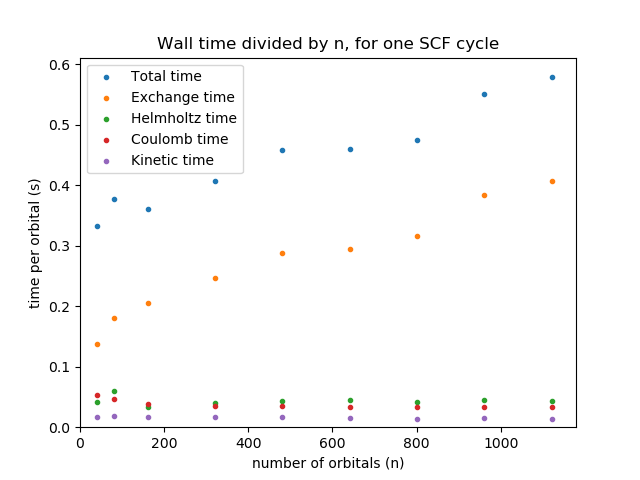
\includegraphics[width=1.\textwidth]{Times_nAlkanes.png}
\caption{\label{fig01}. Computation times divided by number of orbitals for one SCF cycle for different sizes alkanes: $C_{20}H_{42}$, $C_{40}H_{82}$, $C_{80}H_{162}$,$ C_{120}H_{242}$,$ C_{160}H_{322}$,$ C_{200}H_{402}$,$ C_{240}H_{482}$,$ C_{280}H_{562}$. Each molecule is computed using 8 compute nodes. Total time refers to the time spent in one Hartree-Fock SCF cycle, when it is close to convergence. Exchange time refers to the time spent for computing the Exchange contributions. Coulomb time refers to the time used for computing the Coulomb potential of each orbital, summing them up and distributing the total potential to all the compute nodes. Kinetic time refers to the time spent for computing the kinetic energy of each orbital  and Helmholtz time the time for constructing and applying the Helmholtz operator. Constant time per orbital would indicate linear scaling.}
\end{figure}

Figure \ref{fig01} show computation times divided by the number of orbitals for alkanes of different lengths. For a linear scaling method, the time per orbital should be approximately constant.  The time per orbital less than doubles going from the smallest (81 orbitals) to the largest (1121 orbitals) alkane. This shows that the scaling with system size is mostly linear, with a small non-linear contribution.  
% quadratic scaling would multiply the time by 13.8 

%define precisions mw5, mw6 ...

%The time consuming part of the Coulomb potential, is to gather the partial Coulomb potentials from each process, and distribute the total potential to all the processes again. The size (in terms of memory) of the potential will grow linearly with the size of the system. In addition the gather and scatter is done using a binary tree approach in our present implementation (this does not fully exploit the network parallelism, and better schemes can be implemented). The time for the Coulomb calculations is then formally growing as N ln2 N at present. In a local representation, this distribution of the full potential will not be necessary (but this is not yet implemented). At present the Coulomb and nuclear potential are treated independently. Since they largely cancel each other, a better approach would be to consider the sum of them directly, at least for remote nuclei and orbitals.

%The smallest alkanes are not able to make an optimal utilization of all the available cpus

The clearly most time consuming term is the exchange term. The other terms are showing close to linear scaling properties.

The number of non-negligible exchange contributions should ideally grow linearly with system size for large enough systems, and therefore the exchange computation time per orbital should be constant. However exchange contributions are the result of a sum of terms, and if the number of terms increase the accuracy of each individual term must be increased in order to achieve a fixed absolute precision in the final result. In our implementation, this is taking care of by increasing the required precision of the individual terms by a factor proportional to the square root of the number of orbitals. This is the main reason why our run times are not exhibiting a clearer linear trend.


\subsection{Size of orbital representation}
\label{sizes}

In a localized approach, the orbitals functions have negligible values in remote regions of space. In a direct basis set approach (if no special filtering is applied) the representation of an orbital will span the entire represented space, since the basis will increase with the system size. In the MRA approach the orbital will essentially be represented using locally defined functions and their size will depend only weakly on the size of the entire system.
This is confirmed directly in our calculations, see table \ref{tab:orbsizes}.
The individual size of the orbitals, will of course vary greatly according to their type; for example core orbitals are simpler and therefore require less data to represent at a given precision, more diffuse function have more features and require more data to describe. As an illustration, in the molecules presented here, the largest orbital may be two to four times larger than the average, and the smallest a third of the average size.

The number of orbitals together with the size of the orbitals can be seen as an indicator of how much computational resources (memory, cpu time, and network) are required to solve the equations. 

\begin{table*}[t]
    \centering
    \begin{tabular}{cccccccccc}
& $C_{20}H_{42}$& $C_{40}H_{82}$& $C_{80}H_{122}$& $C_{120}H_{242}$&  $C_{200}H_{442}$ & $C_{280}H_{562}$ &valinomycine & gramicidin\\
orbital size (MB)  &  39 &  40   & 43  &  45  & 46 & 47 & 49 & 53\\
    \end{tabular}
    \caption{Average orbital size of different molecules (1e-5 prec). The average orbital size (in terms of number of nodes or coefficients) of the alkanes series is almost independent of the size of the molecule for the largest sizes}
    \label{tab:orbsizes}
\end{table*}



\subsection{Scaling with precision}

In table \ref{tab:prec} we have performed calculations with different precisions on two molecules, valinomycine (300 orbitals) and the gramicidin dimer (1008 orbitals).


\begin{table*}[t]
    \centering
    \begin{tabular}{cccccccccc}
&orbital size& Exchange &  Coulomb & Kinetic energy& Helmholtz & Total \\
 Valinomycine mw5& 49 & 71.4& 9.2& 2.7 & 7.4& 97.4\\
Valinomycine mw6& 115 & 182.4& 25.3& 6.7 & 21.3&251.2\\
Valinomycine mw7& 245 & 442.8& 78.8&17.1& 66.4&644.4  \\
%Valinomycine &1E-8  & 531.0& 163.9& 12.9&32.7& 852.6 \\ older run, different setup
 Gramicidin mw5&55&115&18& 4& 8& 164\\
  Gramicidin mw6&136&312 & 46& 15 & 26& 429\\
  Gramicidin mw7&306& 813&126& 28& 82& 1131\\ %cycle 4
    \end{tabular}
    \caption{Time (in seconds) for different terms in the SCF cycle. Valinomycine using 16 compute nodes and gramicidin 64 compute nodes. The average size (in MB) for one orbital is also given.} %times for cycle 6. 12 MPI/cnode, 4 bank/cnode, 15 OMP
    \label{tab:prec}
 
\end{table*}


An increase in the number of coefficients describing the orbitals will clearly increase the computational cost of each operation using this orbital. In addition an increase in precision will also extend the range of orbitals with non-negligible interactions, i.e. gives less effective screening.
We observe roughly a factor of 2.5 increase in computation time for each increase by a factor of ten of the precision. 



\subsection{Implicit screening} % new
\label{sec:screen}

Since it is at the heart of the MRA approach, we will here show explicitly how the adaptivity of the method leads to a significant reduction of the computation. We will consider linear alkanes of different sizes, as they are is easier to compare.

As first illustration we will consider the evaluation  of the Fock matrix, equation \ref{eq:fock-matrix-definition} using the formulation from equation \ref{equ:sum}

\begin{equation}
\label{equ:sums}
 \braket{\phi_i | {\hat F} |\phi_j}_n = \sum_{k} c_{ikn} d_{jkn} \forall i,j  
\end{equation}

where i and j run over occupied orbitals, n run over all nodes and
k runs over the MW basis within the node, i.e. 3 dimensional polynomials. In the calculations presented in his paper, polynomials up to 7th order in each direction are used, leading to a total of 4096 3-dimensional polynomials (wavelet and scaling) for each node.

 In our implementation, a MW basis which is the union of the basis for all orbitals is defined. This basis can be very large, but we do not define explicitly any function in this basis. In table \ref{tab:adapF} we show the resulting number of nodes defined in this basis (i.e. number of indices n). As expected, the total number of nodes is increasing linearly with system size.
 
 We define a block as one set of {i,j,n} indices. The total number of blocks  is the number of nodes n multiplied by the square of the number of orbitals. For each block equation \ref{equ:sum} defines the multiplication of the corresponding coefficients for all the polynomials defined within a node. The total number of blocks increases with the third power of the system size. However, if a given node is defined for one orbital i, but not for orbital j, this node will not contribute to the corresponding matrix element, and can be neglected. For localized orbitals, i and j will contribute only to local nodes and a large proportion of terms can therefore be neglected before being evaluated explicitly. This is a consequence of the orthogonality of the MW basis.
 
 As shown in table \ref{tab:adapF}, the number of non-negligible terms is still increasing faster than linear. %this means the size of the non-neglected matrices is increasing with system size.
 %something like Nnodes = ax + b(N-x), where x is the number of nodes "close to the edges"; the matrices for  nodes close to the edges are smaller (less neighbors). If N increases, the proportion of large terms increases, for example a doubling of N:
 % (2N-x)/x > (N-x)/x  
 This is not necessarily synonym with computation time increasing faster than linear. To perform the calculations, the code must first fetch the relevant data in the bank, i.e. the matrices $c_{ikn}$ and  $d_{jkn}$ for a fixed n. Then the two matrices are multiplied. As shown in the table the total time used to fetch the data grows slightly slower than linearly. 
 % ? This reflects the fact that the average size of the matrices is increasing with system size: larger matrices will lead to more efficient data transfer. 
 For large systems, the total time to perform the matrix multiplication is proportional to the number of computed terms, and grows faster than linear. On the other hand, the matrix multiplication part is done so efficiently that it takes only a small fraction of the total time. In fact in our implementation we did not even use OpenMP parallelization (yet); an order of magnitude could be gained on the timings for the matrix multiplication part using OpenMP (and even more if GPU accelerators were used). 

%total times do not look good and are therefore not shown; (time for saving in Bank varies a lot). In addition saving might be avoided (moved to other parts) in future versions.
%PW: I do not understand why the computed blocks does not increase towards linear: Isn't  F Psi  local if Psi is local?
\begin{table*}[t]
    \centering
    \begin{tabular}{cccccccccc}
Alkane & Number nodes & blocks&  computed & neglected& time fetch& time multiply\\
$C_{20}H_{42}$   & 6472  &    42462792 &  1558568 & 96.33\% &164 ms & 19 ms\\ 
$C_{40}H_{82}$   & 12936 &   335314056 &  3800528 & 98.86\% &340 ms & 38 ms\\ 
$C_{80}H_{162}$  & 26120 &  2691430920 & 10535312 & 99.61\% &532 ms & 97 ms\\ 
$C_{160}H_{322}$ & 52136 & 21421691816 & 30814576 & 99.85\% &981 ms &270 ms\\ 
    \end{tabular}
    \caption{Number of terms and times to evaluate them in the Fock matrix calculation. Precision MW4. The number of fully computed terms increases faster than linearly, but the fraction of time to perform the corresponding multiplications is small.} %4 compute nodes, 32 MPI workers
    \label{tab:adapF}
\end{table*}


\begin{table*}[t]
    \centering
    \begin{tabular}{cccccccccc}
Alkane & Number of orbitals& non-diagonal terms&  fully computed & fraction neglected \\
$C_{20}H_{42}$ &81 & 3240 & 1146 & 65\% \\ 
$C_{40}H_{82}$ &161 & 12880 & 2548 & 80\% \\ 
$C_{80}H_{162}$ &321 &  51360& 5194& 90\% \\ 
$C_{160}H_{322}$ & 641& 205120 & 10404& 95\% \\ 
    \end{tabular}
    \caption{Number of terms in the Exchange calculation. Precision MW4. The number of terms fully computed becomes proportional to the number of orbitals. } 
    \label{tab:adapEx}
\end{table*}

 
Table \ref{tab:adapEx} shows the total number of exchange terms and how many of them are actually fully computed. Since we exploit the symmetry of the Poisson part, the terms are computed in pairs and the number of pairs non-diagonal terms is $N(N-1)/2$, i.e. scales quadratically.    
The computation of the exchange terms starts with the product of two orbitals. If the product has a norm smaller than a threshold, it can be neglected without having to apply the Poisson operator (which is the computationally expensive part). We see that a large fraction of the terms are effectively neglected, and thereby only the linearly scaling terms are left.



\subsection{Comparison with ORCA  and LSDalton  }

\begin{table*}[t]
    \centering
    \caption{Comparison of results and computation times, for one SCF cycle (Hartree Fock, Valinomycine molecule). LSDalton$^+$ is performed using the accelerators "DENSFIT" and "ADMM". E is the total Hartree fock Energy and $\Delta$E is the atomization energy. The error is defined as the difference with the mw7 results. Time is the wall time per scf cycle. $^*$All computation where done on 4 compute nodes, except for MRChem mw5, mw6 and mw7 which were performed using 16 compute nodes}
    \begin{tabular}{l|cc|cc|r}
    \hline
    \hline
    Program/basis     & E [a.u.]   &Error &$\Delta$E [a.u.]& Error & Time [s]\\
    \hline
    LSDalton/pc-1     &-3770.20554 &2.6e-00 &-19.12076 &1.1e-01 &101     \\
    LSDalton/pc-2     &-3772.56656 &3.0e-01 &-19.27598 &-4.0e-02 &1688    \\
    LSDalton/pc-3     &-3772.83312 &3.3e-02 &-19.24894 &-1.4e-02 &26319   \\
    LSDalton$^+$/pc-3     &-3772.82592 &4.0e-02 &-19.26353 &-2.9e-02 &1924\\
                      &            &        &          &        &        \\
    ORCA/pc-1         &-3770.19956 &2.6e-00 &-19.11479 &1.2e-01 &25      \\
    ORCA/pc-2         &-3772.56922 &3.0e-01 &-19.27865 &-4.4e-02 &265     \\
    ORCA/pc-3         &-3772.83357 &3.2e-02 &-19.24940 &-1.4e-02 &3933    \\
                      &            &        &          &        &        \\
    MRChem/mw4        &-3772.85028 &1.6e-02 &-19.21937 &1.5e-02 &117     \\
    MRChem/mw5        &-3772.86560 &2.5e-04 &-19.23469 &2.5e-04 & 97$^*$ \\
    MRChem/mw6        &-3772.86584 &1.0e-05 &-19.23493 &1.0e-05 &251$^*$ \\
    MRChem/mw7        &-3772.86585 &-       &-19.23494 &-       &644$^*$ \\
    \hline
    \hline
    \end{tabular}    
        \label{tab:MRC_ORCA_LSD}
\end{table*}

Table \ref{tab:MRC_ORCA_LSD} shows the computation time for one SCF cycle for the Valinomycine molecule computed at the Hartree Fock level. The accuracy of the total energy and atomization energies are compared with the ORCA and LSDalton
results using a pc-1, pc-2 and pc-3 basis set (the pc-4 basis was out of reach). 

Even at the lowest precision (mw4), the results have the same quality as the pc-3 basis, but at a fraction of the computational cost. 

It should be stressed that the run times given for ORCA\cite{orca} and LSDalton\cite{lsdalton} could probably be improved by tuning different input parameters, as we did not try to further optimize all the settings. Still the main picture should not be affected.

Note that if the MW results where not available, it would not be easy to estimate the error of the GTO results. The accuracy of a GTO calculation will depend on the choice of basis set, the property of interest and is also affected by BSSE [REF].
The ability to better control precision is a definitive advantage of the MRA method:
The precision is chosen as a single number that can be chosen on a continuous scale. The resulting precision will be independent of the property of interest. %is this true?


\section{Discussion}
%Not ready

We have presented a fully functional implementation of the multiwavelet method and demonstrated that it is capable of handling systems with thousands of electrons at the Hartree Fock (or DFT) level. The methodology results in an almost linear scaling with system size. There are certainly many alternative ways to approach the problem and we still expect that significant improvements in the efficiency of the algorithm will be implemented in the coming years. 

Specially the large memory footprint is a serious bottleneck that should be further addressed. %could be quantified: how large fraction of the coefficients are actually not negligible


It is remarkable that even if the actual basis used in MRChem can be several order of magnitudes larger than what is used in large GTO basis, the computation times are still affordable and even competitive. We believe this is due to the fact that modern computers are extremely efficient when it comes to performing a large number of mathematical operations simultaneously. The parts which are most time consuming are usually the transfer of data from main memory into cache, and transfer of data between compute nodes. The ability to partition the problem into independent parts is becoming more important than minimizing the overall number of mathematical operations. In this respect, the MRA framework has an advantage because of the orthogonality of the initial basis. See also the discussion about the relationship between HPC and Computational Chemistry in \cite{penchoff2021} and \cite{ratcliff2016}.

%GTO methods have been developed at a time where computer power was a scarce resource. In modern computers the total number of mathematical operations that can be performed is huge. For a complex scientific software, the total number of mathematical operations performed will usually be small compared to the maximum theoretically available on a supercomputer. This is even more true for GPU based computers. Therefore the focus of modern software should shift from minimizing the number of operations, towards finding new ways of partitioning the algorithm into independent parts.

For DFT methods, it had already been shown \cite{bischoff2019} MOREREF that MRA methods can be competitive wrt computation time.

For low or medium precision, the computer resources required are still larger than traditional basis set approaches. 



It is fair to say that finite basis set method benefit from decades of development by thousands of scientists, while only a few groups are actually developing multiwavelet methods for quantum chemistry calculations. We can therefore expect that the potential for further optimizations of the method and extension of the range of application will still increase widely in the future.

The advantages of the MRA approach is clearer for large systems and/or high precision. We have shown that such large systems are now affordable on large computers.

%say something about status for correlated methods?


\begin{acknowledgments}
SIGMA2, nn9330k, Hylleraas \dots.
\end{acknowledgments}




%\bibliographystyle{plain}
%\bibliography{references}

%Goedecker, S. (1999). Linear scaling electronic structure methods. Reviews of Modern Physics, 71(4), 1085–1123. doi:10.1103/revmodphys.71.1085 

%Real space methods:
% DOI: 10.1039/C5CP90198G (Editorial) Phys. Chem. Chem. Phys., 2015, 17, 31357-31359
%Real-space numerical grid methods in quantum chemistry
%Luca Frediani and Dage Sundholm
%https://pubs.rsc.org/en/content/articlehtml/2015/cp/c5cp90198g?page=search


%https://pubs.rsc.org/en/journals/journalissues/cp#!issueid=cp017047&type=current&issnprint=1463-9076

%MP2:
%https://aip.scitation.org/doi/10.1063/1.5141880
%Direct determination of optimal pair-natural orbitals in a real-space representation: The second-order Moller–Plesset energy
% J. Chem. Phys. 152, 074105 (2020); https://doi.org/10.1063/1.5141880
%Jakob S. Kottmann1,a), Florian A. Bischoff1,b), and Edward F. Valeev

%Predictive computation of properties of molecules and materials requires a highly precise numerical representation of many-body electronic wave functions/operators. Accurate electronic wave functions, such as in the coupled-cluster method, are traditionally represented in the Linear Combination of Atomic Orbitals (LCAO) representation using pre-optimized sequences of atom-centered basis sets (represented by analytic Gaussian-type or Slater-type functions, or represented numerically1). Recently, many-body electronic structure computations have also been demonstrated in the (augmented) plane-wave (PW) representation.2 Both representations suffer from slow convergence to the basis set limit, requiring the use of basis set extrapolation3,4 or explicit correlation.5,6 Although it is possible to closely match experimental chemical energy differences, such as atomization energies of small molecules,7 with the LCAO approaches, such computations suffer from high cost and poor conditioning and do not lend themselves to fast (reduced-scaling) reformulation due to the fully dense representation of electronic states and operators. The known bias of common AO basis sets toward ground-state energies makes it difficult to attain similar accuracy for excited states and response properties. Meanwhile, the plane wave representation struggles with the description of position-localized (e.g., intra-atomic) features of the electronic wave functions and thus also do not naturally lend themselves to low-order formulations.
%Grid-based real-space numerical representations of many-body wave functions, such as finite difference and finite/spectral elements, provide an alternative to the LCAO and PW representations with a number of attractive features, such as the ability to resolve spatially localized features, systematic bias-free improvability, and good conditioning. The main bottleneck to routine use of such representations is the impractical size of the 3k-dimensional grid needed to represent a k-particle state. Even pair theories (k = 2) such as MP2 and CCSD become prohibitively expensive for molecular systems due to the grid size; only symmetry-based dimension reduction in atoms makes the application of pair theories possible.8–12

\begin{thebibliography}{}


\bibitem[Bischoff (2019)]{bischoff2019}Florian A. Bischoff https://doi.org/10.1016/bs.aiq.2019.04.003  Computing accurate molecular properties in real space using multiresolution analysis,  2019

\bibitem[Ratcliff (2020)]{ratcliff2020}Laura E. Ratcliff,  William Dawson2, Giuseppe Fisicaro, Damien Caliste, Stephan Mohr, Augustin Degomme, Brice Videau, Viviana Cristiglio, Martina Stella, Marco D’Alessandro, Stefan Goedecker, Takahito Nakajima2, Thierry Deutsch, and Luigi Genovese J. Chem. Phys. 152, 194110 (2020) https://doi.org/10.1063/5.0004792 Flexibilities of wavelets as a computational basis set for large-scale electronic structure calculations

\bibitem[Harrison (2016)]{madness2016}R. J. Harrison, G. Beylkin, F. A. Bischoff, J. A. Calvin, G. I. Fann, J. Fosso-Tande, D. Galindo, J. R. Hammond, R. Hartman-Baker, J. C. Hill, J. Jia, J. S. Kottmann, M.-J. Yvonne Ou, J. Pei, L. E. Ratcliff, M. G. Reuter, A. C. Richie-Halford, N. A. Romero, H. Sekino, W. A. Shelton, B. E. Sundahl, W. S. Thornton, E. F. Valeev, Á. Vázquez-Mayagoitia, N. Vence, T. Yanai, and Y. Yokoi, SIAM J. Sci. Comput. 38, S123 (2016). https://doi.org/10.1137/15m1026171

\bibitem[Ratcliff (2016)]{ratcliff2016}Laura E. Ratcliff, Stephan Mohr, Georg Huhs, Thierry Deutsch, Michel Masella, Luigi Genovese  https://doi.org/10.1002/wcms.1290 Challenges in large scale quantum mechanical calculations

\bibitem[Helgaker (2000)]{trygve},T. Helgaker, P. Jørgensen, and J. Olsen., Molecular Electronic‐Structure Theory  John Wiley \& Sons, LTD, Chichester (2000)

\bibitem[penchoff (2021)]{penchoff2021} https://pubs.acs.org/doi/full/10.1021/bk-2021-1388.ch001  HPC challenges: An Introduction to High Performance Computing and Its Intersection with Advances in Modeling Rare Earth Elements and Actinides
 
\bibitem[ORCA (2020)]{orca} F. Neese, F. Wennmohs, U. Becker, and C. Riplinger, “The ORCA quantum chemistry program package”, J. Chem. Phys. 152, 224108 (2020). https://doi.org/10.1063/5.0004608
 
\bibitem[LSDalton (2014)]{lsdalton} K. Aidas, C. Angeli, K. L. Bak, V. Bakken, R. Bast, L. Boman, O. Christiansen, R. Cimiraglia, S. Coriani, P. Dahle, E. K. Dalskov, U. Ekström, T. Enevoldsen, J. J. Eriksen, P. Ettenhuber, B. Fernández, L. Ferrighi, H. Fliegl, L. Frediani, K. Hald, A. Halkier, C. Hättig, H. Heiberg, T. Helgaker, A. C. Hennum, H. Hettema, E. Hjertenæs, S. Høst, I.-M. Høyvik, M. F. Iozzi, B. Jansik, H. J. Aa. Jensen, D. Jonsson, P. Jørgensen, J. Kauczor, S. Kirpekar, T. Kjærgaard, W. Klopper, S. Knecht, R. Kobayashi, H. Koch, J. Kongsted, A. Krapp, K. Kristensen, A. Ligabue, O. B. Lutnæs, J. I. Melo, K. V. Mikkelsen, R. H. Myhre, C. Neiss, C. B. Nielsen, P. Norman, J. Olsen, J. M. H. Olsen, A. Osted, M. J. Packer, F. Pawlowski, T. B. Pedersen, P. F. Provasi, S. Reine, Z. Rinkevicius, T. A. Ruden, K. Ruud, V. Rybkin, P. Salek, C. C. M. Samson, A. Sánchez de Merás, T. Saue, S. P. A. Sauer, B. Schimmelpfennig, K. Sneskov, A. H. Steindal, K. O. Sylvester-Hvid, P. R. Taylor, A. M. Teale, E. I. Tellgren, D. P. Tew, A. J. Thorvaldsen, L. Thøgersen, O. Vahtras, M. A. Watson, D. J. D. Wilson, M. Ziolkowski, and H. Ågren, "The Dalton quantum chemistry program system", WIREs Comput. Mol. Sci. 2014, 4:269–284 (doi:10.1002/wcms.1172)

\bibitem[MPI3]{mpi}Message Passing Interface Forum, "MPI: A Message-Passing Interface Standard Version 3.1", (2015). https://www.mpi-forum.org/docs/mpi-3.1/mpi31-report.pdf

\bibitem[OpenMP]{omp} https://www.openmp.org

\end{thebibliography}
\end{document}
